% ----------------------------------------------------------------
% AMS-LaTeX Paper ************************************************
% **** -----------------------------------------------------------
%\documentclass{amsart}
%\usepackage{txfonts}
%\documentclass[12pt,oneside]{article}
\documentclass{amsart}
\usepackage{graphicx}
\usepackage{enumitem}
% ----------------------------------------------------------------
\vfuzz2pt % Don't report over-full v-boxes if over-edge is small
\hfuzz2pt % Don't report over-full h-boxes if over-edge is small
% THEOREMS -------------------------------------------------------
\newtheorem{thm}{Theorem}[section]
\newtheorem{cor}[thm]{Corollary}
\newtheorem{lem}[thm]{Lemma}
\newtheorem{prop}[thm]{Proposition}
\theoremstyle{definition}
\newtheorem{defn}[thm]{Definition}
\theoremstyle{Exercise}
\newtheorem{ex}[thm]{Exercise}
\theoremstyle{remark}
\newtheorem{rem}[thm]{Remark}
\theoremstyle{rule}
\newtheorem{rul}[thm]{Rule}

\numberwithin{equation}{section}
% MATH -----------------------------------------------------------
\newcommand{\norm}[1]{\left\Vert#1\right\Vert}
\newcommand{\abs}[1]{\left\vert#1\right\vert}
\newcommand{\set}[1]{\left\{#1\right\}}
\newcommand{\Real}{\mathbb R}
\newcommand{\Z}{\mathbb Z}
\newcommand{\To}{\longrightarrow}
\newcommand{\BX}{\bB(X)}
\newcommand{\A}{\mathcal{A}}
% ----------------------------------------------------------------

% define some simple, commonly-used commands
\newcommand{\eps}{\varepsilon}
\newcommand{\dsum}{\displaystyle\sum}
\newcommand{\dint}{\displaystyle\int}

\newcommand{\pdr}[2]{\dfrac{\partial{#1}}{\partial{#2}}}
\newcommand{\pdrr}[2]{\dfrac{\partial^2{#1}}{\partial{#2}^2}}
\newcommand{\pdrt}[3]{\dfrac{\partial^2{#1}}{\partial{#2}{\partial{#3}}}}
\newcommand{\dr}[2]{\dfrac{d{#1}}{d{#2}}}
\newcommand{\aver}[1]{\langle {#1} \rangle}
\newcommand{\Baver}[1]{\Big\langle {#1} \Big\rangle}

\newcommand{\bzero}{\mathbf 0}
\newcommand{\bGamma}{\mbox{\boldmath{$\Gamma$}}}
\newcommand{\btheta}{\boldsymbol \theta}
\newcommand{\bchi}{\mbox{\boldmath{$\chi$}}}
\newcommand{\bnu}{\boldsymbol \nu}
\newcommand{\bmu}{\boldsymbol \mu}
\newcommand{\brho}{\mbox{\boldmath{$\rho$}}}
\newcommand{\bxi}{\boldsymbol \xi}
\newcommand{\bnabla}{\boldsymbol \nabla}
\newcommand{\bOm}{\boldsymbol \Omega}
\newcommand{\blambda}{\boldsymbol \lambda}
\newcommand{\bsigma}{\boldsymbol \sigma}

\newcommand{\bbR}{\mathbb R}
\newcommand{\bbC}{\mathbb C}
\newcommand{\bbQ}{\mathbb Q}
\newcommand{\bbN}{\mathbb N}
\newcommand{\bbZ}{\mathbb Z}

\newcommand{\ba}{\mathbf a} \newcommand{\bb}{\mathbf b}
\newcommand{\bc}{\mathbf c} \newcommand{\bd}{\mathbf d}
\newcommand{\be}{\mathbf e} \newcommand{\bff}{\mathbf f}
\newcommand{\bg}{\mathbf g} \newcommand{\bh}{\mathbf h}
\newcommand{\bi}{\mathbf i} \newcommand{\bj}{\mathbf j}
\newcommand{\bk}{\mathbf k} \newcommand{\bl}{\mathbf l}
\newcommand{\bm}{\mathbf m} \newcommand{\bn}{\mathbf n}
\newcommand{\bo}{\mathbf o} \newcommand{\bp}{\mathbf p}
\newcommand{\bq}{\mathbf q} \newcommand{\br}{\mathbf r}
\newcommand{\bs}{\mathbf s} \newcommand{\bt}{\mathbf t}
\newcommand{\bu}{\mathbf u} \newcommand{\bv}{\mathbf v}
\newcommand{\bw}{\mathbf w} \newcommand{\bx}{\mathbf x}
\newcommand{\by}{\mathbf y} \newcommand{\bz}{\mathbf z}
\newcommand{\bA}{\mathbf A} \newcommand{\bB}{\mathbf B}
\newcommand{\bC}{\mathbf C} \newcommand{\bD}{\mathbf D}
\newcommand{\bE}{\mathbf E} \newcommand{\bF}{\mathbf F}
\newcommand{\bG}{\mathbf G} \newcommand{\bH}{\mathbf H}
\newcommand{\bI}{\mathbf I} \newcommand{\bJ}{\mathbf J}
\newcommand{\bK}{\mathbf K} \newcommand{\bL}{\mathbf L}
\newcommand{\bM}{\mathbf M} \newcommand{\bN}{\mathbf N}
\newcommand{\bO}{\mathbf O} \newcommand{\bP}{\mathbf P}
\newcommand{\bQ}{\mathbf Q} \newcommand{\bR}{\mathbf R}
\newcommand{\bS}{\mathbf S} \newcommand{\bT}{\mathbf T}
\newcommand{\bU}{\mathbf U} \newcommand{\bV}{\mathbf V}
\newcommand{\bW}{\mathbf W} \newcommand{\bX}{\mathbf X}
\newcommand{\bY}{\mathbf Y} \newcommand{\bZ}{\mathbf Z}

\newcommand{\cA}{\mathcal A} \newcommand{\cB}{\mathcal B}
\newcommand{\cC}{\mathcal C} \newcommand{\cD}{\mathcal D}
\newcommand{\cE}{\mathcal E} \newcommand{\cF}{\mathcal F}
\newcommand{\cG}{\mathcal G} \newcommand{\cH}{\mathcal H}
\newcommand{\cI}{\mathcal I} \newcommand{\cJ}{\mathcal J}
\newcommand{\cK}{\mathcal K} \newcommand{\cL}{\mathcal L}
\newcommand{\cM}{\mathcal M} \newcommand{\cN}{\mathcal N}
\newcommand{\cO}{\mathcal O} \newcommand{\cP}{\mathcal P}
\newcommand{\cQ}{\mathcal Q} \newcommand{\cR}{\mathcal R}
\newcommand{\cS}{\mathcal S} \newcommand{\cT}{\mathcal T}
\newcommand{\cU}{\mathcal U} \newcommand{\cV}{\mathcal V}
\newcommand{\cW}{\mathcal W} \newcommand{\cX}{\mathcal X}
\newcommand{\cY}{\mathcal Y} \newcommand{\cZ}{\mathcal Z}


%%%%%%%%%%%%%%Start%%%%%%%%%%%%%Start%%%%%%%%%%%Start%%%%%%%%%%%%%%%Start%%%%%%%%%%%%%%%%%%%%%%%%%Start%%%%%%%%%%%%%%%%
%%%%%%%%%%%%%%Start%%%%%%%%%%%%%Start%%%%%%%%%%%Start%%%%%%%%%%%%%%%Start%%%%%%%%%%%%%%%%%%%%%%%%%Start%%%%%%%%%%%%%%%%
%%%%%%%%%%%%%%Start%%%%%%%%%%%%%Start%%%%%%%%%%%Start%%%%%%%%%%%%%%%Start%%%%%%%%%%%%%%%%%%%%%%%%%Start%%%%%%%%%%%%%%%%
\usepackage{xcolor}
\usepackage{fancyhdr}

\pagestyle{fancy}
\fancyhf{}
\rhead{}
\chead{
\includegraphics[scale=.1]{snhu_logo.png}}

\begin{document}
\begin{center}

\includegraphics[scale=.1]{snhu_logo.png}
\end{center}
\title{\sf Module Five Problem Set}%


%\thm{bbjh}
\maketitle
This document is proprietary to Southern New Hampshire University. It and the problems within may not be posted on any non-SNHU website.\\\\\\\\
\begin{center}
%Enter your name below this line:
Brad Jackson
\end{center}


\begin{center}
\rule{\textwidth}{0.4pt}
\end{center}


\newpage

%--------------------------------------------------------------------------------------------------
\section*{}
\section*{}
Directions: Type your solutions into this document and be sure to show all steps for arriving at your solution. Just giving a final number may not receive full credit.
\\\\
\section*{Problem 1}

Indicate whether the two functions are equal. If the two functions are not equal, then give an element of the domain on which the two functions have different values.\\
 \begin{enumerate}[label=(\alph*)]
   \item
\[ f: \Z \to \Z, \text{ where } f(x)= x^2.\]
\[ g: \Z \to \Z, \text{ where } g(x)= |x|^2.\]\\\\
%Enter your answer below this comment line.
Functions $f$ and $g$ have the same domain and target.\\
Moreover, for any integer $x$, $x^2 = |x|^2$\\
$f = g$\\
\\\\
\item  \[ f: \Z\times \Z \to \Z, \text{ where } f(x,y)= |x+y|.\]
\[ g: \Z\times \Z \to \Z, \text{ where } g(x,y)= |x|+|y|.\]\\\\
%Enter your answer below this comment line.
Functions f and g have the same domain and target.\\
Moreover, for each ordered pair of integers $x$ and $y$, $|x+y| = |x|+|y|$\\
\\\\
\end{enumerate}

 \newpage
%--------------------------------------------------------------------------------------------------

\section*{Problem 2}

The domain and target set of functions f and g is $\mathbb{R}$. The functions are defined as:
\begin{itemize}
  \item $f(x) = 2x + 3$\\

  \item $g(x) = 5x + 7$\\


\end{itemize}

\begin{enumerate}[label=(\alph*)]
\item  $f\circ g$?\\\\
%Enter your answer below this comment line.
$2(5x+7)+3$\\
$10x+17$\\
\\\\
\item  $g \circ f$?\\\\
%Enter your answer below this comment line.
$10x+22$\\
\\\\
\item  $(f\circ g)^{-1}$?\\\\
%Enter your answer below this comment line.
$(x-17)/10$\\
\\\\
\item  $f^{-1}\circ g^{-1}$?\\\\
%Enter your answer below this comment line.
$(x-3)/2$\\
\\\\
\item  $g^{-1}\circ f^{-1}$?\\\\
%Enter your answer below this comment line.
$(x-22)/10$\\
\\\\
\end{enumerate}
Are any of the above equal?\\\\
%Enter your answer below this comment line.
None of the above are equal.
\\\\


    \newpage
%--------------------------------------------------------------------------------------------------



\section*{Problem 3}

\begin{enumerate}[label=(\alph*)]
\item  Give the matrix representation for the relation depicted in the arrow diagram. Then, express the relation as a set of ordered pairs.\\\\
The arrow diagram below represents a relation.\\
\fbox{
 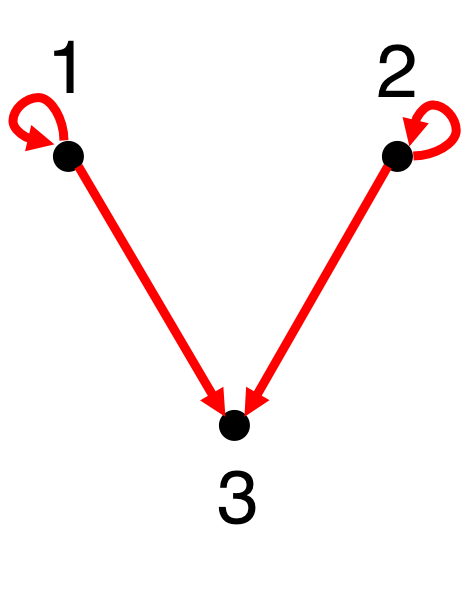
\includegraphics[width=2in]{M5-fig1}
}\\\\
{\color{blue}{\bf Figure 1:} \emph{An arrow diagram shows three vertices, 1, 2, and 3. An arrow from vertex 1 points to vertex 3, and another arrow from vertex 2 points to vertex 3. Two self loops are formed, one at vertex 1 and another at vertex 2. 
}
}
\\\\
%Enter your answer below this comment line.
%For more information on creating matrices in LaTeX, see this week's module resources.
\begin{matrix}
  1 & 0 & 1\\
  0 & 1 & 1\\
  0 & 0 & 0\\
  \end{matrix}\\
R = {(1,1)(1,3)(2,2)(2,3)}
\\

\item Draw the arrow diagram for the relation.\\
 The domain for the relation $A$ is the set $\{2,\, 5,\, 7,\, 8,\, 11\}$. For $x$, $y$ in the domain, $xAy$ if $|x-y|$ is less than $2$.
\\\\
%Enter your answer below this comment line.

%To answer this question, you may hand-draw your solution or use a program like PowerPoint or Lucidchart.
%Take a photo or screenshot, then upload your file to this project. Note that the image you submit must be legible to your instructor.
%You will see your file name appear in the file tree. Change the "YOURFILENAMEHERE" text in the includegraphics command below. It should match the name of your uploaded file.

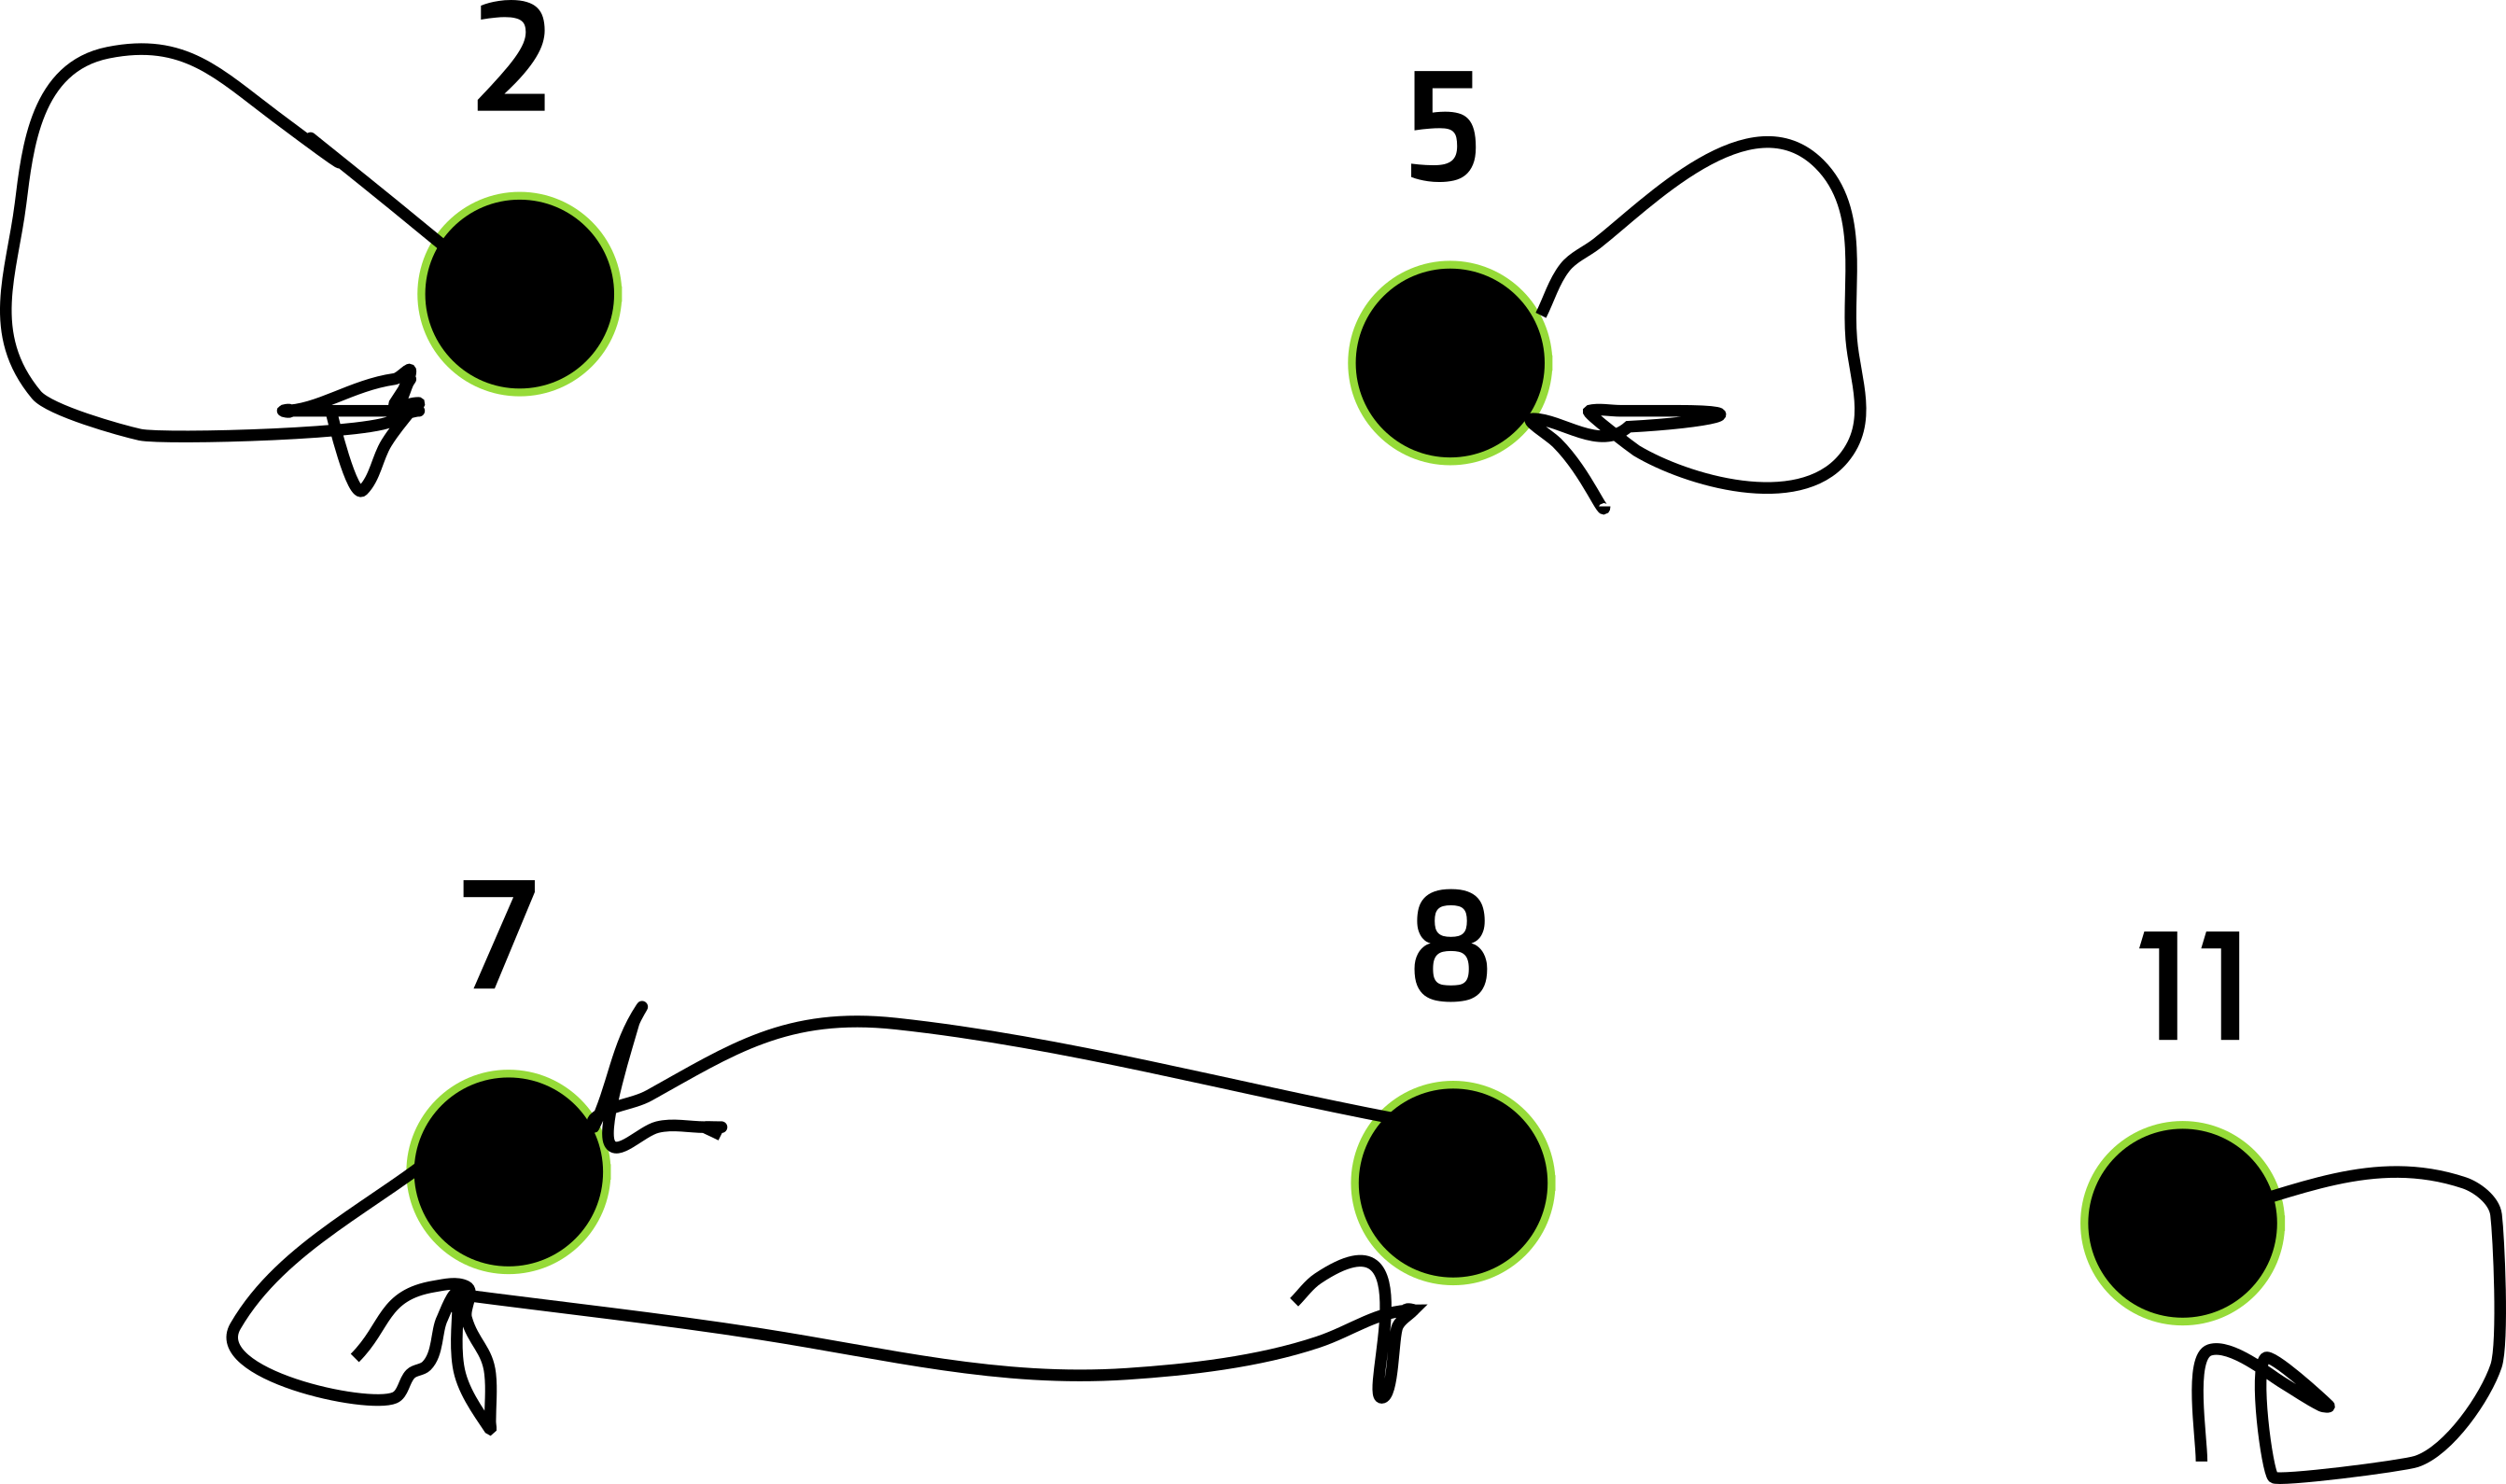
\includegraphics[width=2in]{3333.png}
\\\\
\end{enumerate}
 \newpage
%--------------------------------------------------------------------------------------------------

\section*{Problem 4}

For each relation, indicate whether the relation is:
\begin{itemize}
  \item Reflexive, anti-reflexive, or neither
  \item Symmetric, anti-symmetric, or neither
  \item Transitive or not transitive
\end{itemize}
Justify your answer.\\
\begin{enumerate}[label=(\alph*)]
\item The domain of the relation $L$ is the set of all real numbers. For $x$, $y \in \Real, \; xLy$ if $x < y$.\\\\
%Enter your answer below this comment line.
L is anti-reflexive and transitive:\\

\\\\

\item The domain of the relation $A$ is the set of all real numbers. $xAy$ if $|x-y| \leq 2$\\\\
%Enter your answer below this comment line.
reflexive, symmetric, transitive
\\\\
\item The domain of the relation $Z$ is the set of all real numbers. $xZy$ if $y=2x$\\\\\\\\
%Enter your answer below this comment line.
\\\\
\end{enumerate}
\newpage
\section*{Problem 5}

The number of watermelons in a truck are all weighed on a scale. The scale rounds the weight of every watermelon to the nearest pound. The number of pounds read off the scale for each watermelon is called its measured weight. The domain for each of the following relations below is the set of watermelons on the truck. For each relation, indicate whether the relation is:
\\
\begin{itemize}
  \item Reflexive, anti-reflexive, or neither
  \item Symmetric, anti-symmetric, or neither
  \item Transitive or not transitive
\end{itemize}
Justify your answer.\\

\begin{enumerate}[label=(\alph*)]
\item Watermelon $x$ is related to watermelon $y$ if the measured weight of watermelon $x$ is at least the measured weight of watermelon $y$. No two watermelons have the same measured weight.\\\\
%Enter your answer below this comment line.
Reflexive because $x$ is related to $y$.\\
Anti-symmetric because no two watermelons have the same weight.\\
Not transitive because $z$ could be greater than $x$ as all watermelons do not have the same weight.
\\\\
\item Watermelon $x$ is related to watermelon $y$ if the measured weight of watermelon $x$ is at least the measured weight of watermelon $y$. All watermelons have exactly the same measured weight.\\\\
%Enter your answer below this comment line.
Reflexive because  $x \geq y$, therefore $x$ is related to $y$.\\
Symmetric because all watermelons have the same weight.\\
Transitive because $x \geq y$ then $x \geq z$
\\\\
\end{enumerate}
 \newpage
%--------------------------------------------------------------------------------------------------

\section*{Problem 6}
\subsection*{Part 1}
Give the adjacency matrix for the graph G as pictured below:\\
\\
\fbox{
 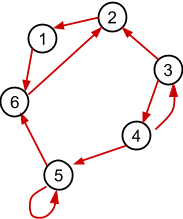
\includegraphics[width=1.75in]{M5-fig2}\\
}\\\\
{\color{blue}{\bf Figure 2:} \emph{A graph shows 6 vertices and 9 edges. The vertices are 1, 2, 3, 4, 5, and 6, represented by circles. The edges between the vertices are represented by arrows, as follows: 4 to 3; 3 to 2; 2 to 1; 1 to 6; 6 to 2; 3 to 4; 4 to 5; 5 to 6; and a self loop on vertex 5.
}
}\\
%Enter your answer below this comment line.
%For more information on creating matrices in LaTeX, see this week's module resources.
\begin{matrix}
  0 & 0 & 0 & 0 & 0 & 1\\
  1 & 0 & 0 & 0 & 0 & 0\\
  0 & 1 & 0 & 1 & 0 & 0\\
  0 & 0 & 1 & 0 & 1 & 0\\
  0 & 0 & 0 & 0 & 1 & 1\\
  0 & 1 & 0 & 0 & 0 & 0\\
  \end{matrix}\\
\\\\

\subsection*{Part 2}
A directed graph $G$ has 5 vertices, numbered 1 through 5. The $5\times 5$ matrix $A$ is the adjacency matrix for $G$. The matrices $A^2$ and $A^3$ are given below.
\[
A^2  = \left( \begin{array}{ccccc}
0 & 1 & 0 & 0 & 0 \\
0 & 0 & 1 & 0 & 0\\
1 & 0 & 0 & 0 & 0\\
1 & 0 & 0 & 1 & 0\\
0 & 1 & 1 & 0 & 1
\end{array} \right)~~~~~~~
\]
\[
A^3  = \left( \begin{array}{ccccc}
1 & 0 & 0 & 0 & 0 \\
0 & 1 & 0 & 0 & 0\\
0 & 0 & 1 & 0 & 0\\
0 & 1 & 1 & 0 & 1\\
1 & 1 & 0 & 1 & 0
\end{array} \right)~~~~~~~
\]
Use the information given to answer the questions about the graph G.
\begin{enumerate}[label=(\alph*)]
\item Which vertices can reach vertex 2 by a walk of length 3?\\\\
%Enter your answer below this comment line.
2, 4, and 5
\\\\

\item Is there a walk of length 4 from vertex 4 to vertex 5 in $G$? (Hint: $A^4 = A^2\cdot A^2$.)\\\\
%Enter your answer below this comment line.
No, shown by the adjacency matrix below.
\[
A^4  = \left( \begin{array}{ccccc}
0 & 1 & 0 & 0 & 0 \\
0 & 0 & 1 & 0 & 0\\
1 & 0 & 0 & 0 & 0\\
1 & 0 & 0 & 1 & 0\\
0 & 1 & 1 & 0 & 1
\end{array} \right)~~~~~~~
\]
\end{enumerate}

 \newpage
%--------------------------------------------------------------------------------------------------

\section*{Problem 7}
\subsection*{Part 1} The drawing below shows a Hasse diagram for a partial order on the set $\{A,\, B,\, C,\, D,\, E,\, F,\, G,\, H,\, I,\, J\}$
\\
\\
\fbox{
 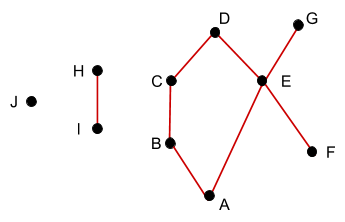
\includegraphics[width=2in]{M5-fig3}\\
}\\
\\
{\color{blue}{\bf Figure 3:} \emph{A Hasse diagram shows 10 vertices and 8 edges. The vertices, represented by dots, are as follows: vertex J; vertices H and I are aligned vertically to the right of vertex J; vertices A, B, C, D, and E forms a closed loop, which is to the right of vertices H and I; vertex G is inclined upward to the right of vertex E; and vertex F is inclined downward to the right of vertex E. The edges, represented by line segments, between the vertices are as follows: Vertex J is connected to no vertex; a vertical edge connects vertices H and I; a vertical edge connects vertices B and C; and 6 inclined edges connect the following vertices, A and B, C and D, D and E, A and E, E and G, and E and F.
}
}
\\
\\

\begin{enumerate}[label=(\alph*)]
\item What are the minimal elements of the partial order?\\\\
%Enter your answer below this comment line.
I, A, and F
\\\\

\item What are the maximal elements of the partial order?\\\\
%Enter your answer below this comment line.
H, D, and G
\\\\

\item Which of the following pairs are comparable?\\
\[
(A, \,D),\, (J,\, F),\, (B,\, E),\, (G, \,F),\, (D,\, B),\, (C, \,F),\, (H,\, I), \,(C,\, E)
\]\\\\
%Enter your answer below this comment line.
(C,E)
\\\\

\end{enumerate}

\subsection*{Part 2}
Each relation given below is a partial order. Draw the Hasse diagram for the partial order.

\begin{enumerate}[label=(\alph*)]
\item The domain is $\{3,\, 5,\, 6,\, 7,\, 10,\, 14,\, 20,\, 30,\, 60\}$. $x \leq y$ if $x$ evenly divides $y$.\\\\
%Enter your answer below this comment line.

%To answer this question, you may hand-draw your solution or use a program like PowerPoint or Lucidchart.
%Take a photo or screenshot, then upload your file to this project. Note that the image you submit must be legible to your instructor.
%You will see your file name appear in the file tree. Change the "YOURFILENAMEHERE" text in the includegraphics command below. It should match the name of your uploaded file.
\includegraphics[width=2in]{YOURFILENAMEHERE}
\\\\

\item The domain is $\{a,\, b,\, c,\, d,\, e,\, f\}$. The relation is the set:
\[
\{ (b,\, e),\, (b,\, d),\, (c,\, a),\, (c,\, f),\, (a,\, f),\, (a,\, a),\, (b,\, b),\, (c, \,c),\, (d,\, d),\, (e, \,e), \,(f,\, f) \}
\]\\\\
%Enter your answer below this comment line.

%To answer this question, you may hand-draw your solution or use a program like PowerPoint or Lucidchart.
%Take a photo or screenshot, then upload your file to this project. Note that the image you submit must be legible to your instructor.
%You will see your file name appear in the file tree. Change the "YOURFILENAMEHERE" text in the includegraphics command below. It should match the name of your uploaded file.
\includegraphics[width=2in]{YOURFILENAMEHERE}
\\\\

\end{enumerate}

\newpage%--------------------------------------------------------------------------------------------------

\section*{Problem 8}

Determine whether each relation is an equivalence relation. Justify your answer. If the relation is an equivalence relation, then describe the partition defined by the equivalence classes.\\
\begin{enumerate}[label=(\alph*)]
\item The domain is a group of people. Person $x$ is related to person $y$ under relation $M$ if $x$ and $y$ have the same favorite color. You can assume that there is at least one pair in the group, $x$ and $y$, such that $xMy$.\\\\
%Enter your answer below this comment line.
\\\\

\item The domain is the set of all integers. $xEy$ if $x + y$ is even. An integer $z$ is even if $z = 2k$ for some integer $k$.\\\\
%Enter your answer below this comment line.
\\\\

\end{enumerate}
%--------------------------------------------------------------------------------------------------



\end{document}
